\scanpage{45}
\mspage{\handwritten{13}}
il suffit de voir que si $\handwritten{\mathcal{F}}$ est plat sur $\handwritten{\mathcal{O}}_S$, \inserted{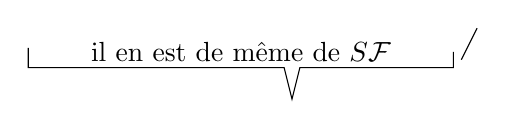
\begin{tikzpicture}[x=1cm,y=1cm,baseline=(n.base)]\node (n) at (0,0) {il en est de même de $\handwritten{\mathbb{S}\mathcal{F}}$};\draw (-2.7,.05)--(-2.7,-.2)--(.55,-.2)--(.65,-.6)--(.75,-.2)--(2.7,-.2)--(2.7,0);\draw (2.8,-.1)--(3,.3);\end{tikzpicture}} ce qui \deleted{résulte des définitions (EGA II 1.7.1), compte tenu d'}\inserted{\handwritten{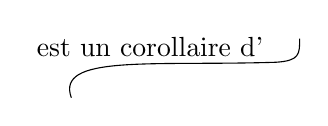
\begin{tikzpicture}[x=1cm,y=1cm,baseline=(n.base)]\node (n) at (0,0) {est un corollaire d'};\draw (-1,-.65) .. controls (-1.2,-.1) and (0,-.25) .. (1.6,-.2) .. controls (1.9,-.18) and (1.9,-.1) .. (1.9,.1);\end{tikzpicture}}}un resultat dû à Daniel LAZARD, suivant lequel tout\deleted{e limite inductive de modules plats est un} module plat\deleted{.} \inserted{\handwritten{sur un anneau est une limite inductive filtrante de modules libres de type fini.}}

\deleted{Remarquons de plus que $\handwritten{\unsure{\mathcal{A}|a}}(X)\handwritten{\otimes}_{\handwritten{\mathcal{O}}_S}\handwritten{\mathbb{S}\mathcal{F}}=\handwritten{\mathbb{S}}(\handwritten{\mathcal{A}}(X)\handwritten{\otimes}_{\handwritten{\mathcal{O}}_S}\handwritten{\mathcal{F}})$ d'après (EGA II 1.1.2), ce qui montre que l'homomorphisme canonique $\handwritten{\mathcal{A}}(X)\handwritten{\otimes}_{\handwritten{\mathcal{O}}_S}\handwritten{\mathcal{F}\longrightarrow}\deleted{\handwritten{\mathbb{S}}}\handwritten{\mathcal{A}}(X)\handwritten{\otimes}_{\handwritten{\mathcal{O}}_S}\handwritten{\mathbb{S}\mathcal{F}}\deleted{\unsure{)}}$ est injectif.}

Montrons maintenant ii). Soit $\handwritten{\alpha}$ un morphisme de $S$-foncteurs de $X$ dans $\handwritten{\mathcal{H}om}_{\handwritten{\mathcal{O}}_S}(\handwritten{\mathbb{V}}(\handwritten{\mathcal{F}}),\handwritten{\mathbb{V}}(\handwritten{\mathcal{E}}))$; il lui correspond un homomorphisme $\handwritten{\rho}$ de $\handwritten{\mathcal{O}}_S$-Modules de $\handwritten{\mathcal{E}}$ dans $\handwritten{\mathcal{A}}(X\handwritten{\times}_S\handwritten{\mathbb{V}}(\handwritten{\mathcal{F}}))=\handwritten{\mathcal{A}}(X)\handwritten{\otimes}_{\handwritten{\mathcal{O}}_S}\handwritten{\mathbb{S}}(\handwritten{\mathcal{F}})$ tel que si $\handwritten{\rho}$ est une $S$-section de $X$, l'homomorphisme
\[
(\handwritten{\mathcal{A}(\eta)\otimes}\operatorname{id}_{\handwritten{\mathbb{S}\mathcal{F}}})\handwritten{\unsure{o|\circ}\rho}:\handwritten{\mathcal{E}\longrightarrow\mathcal{O}}_S\handwritten{\otimes}_{\handwritten{\mathcal{O}}_S}\handwritten{\mathbb{S}\mathcal{F}=\mathbb{S}\mathcal{F}}
\]
corresponde à $\handwritten{\alpha(\eta)}$. Mais puisque $\handwritten{\alpha(\eta)\in}\deleted{\handwritten{\unsure{\mathcal{E}|\mathcal{H}om}}}\handwritten{\mathcal{H}om}_{\handwritten{\mathcal{O}}_S}(\handwritten{\mathbb{V}}(\handwritten{\mathcal{F}}),\handwritten{\mathbb{V}}(\handwritten{\mathcal{E}}))(S)$, $\handwritten{\mathcal{A}(\eta)\otimes}\operatorname{id}_{\handwritten{\mathbb{S}\mathcal{F}}}$ se factorise à travers l'homomorphisme canonique injectif $\handwritten{\mathcal{F}\to\mathbb{S}\mathcal{F}}$. On a donc, pour chaque $S$-section $\handwritten{\eta}$ de $X$\handwritten{,}un diagramme commutatif :
\margin{\handwritten{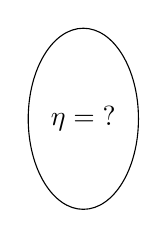
\begin{tikzpicture}
\draw (0,0) ellipse (.7 and 1.15);
\node at (0,0) {$\eta={?}$};
\end{tikzpicture}}}
\diagram{\handwritten{\begin{tikzcd}[ampersand replacement=\&]
\mathcal{E}\arrow[r,"\rho"]\arrow[d]\arrow[d,no head,shift left=1.2pt,shorten >=3pt] \& \mathcal{A}(X)\otimes\mathbb{S}\mathcal{F}\arrow[d]\arrow[dl,"\mathcal{A}(\eta)\otimes\operatorname{id}"']\\
\mathbb{S}\mathcal{F} \& \mathcal{F}\arrow[l]
\end{tikzcd}}}
\handwritten{,}

ce qui montre que $\handwritten{\rho}$ se factorise à travers l'homomorphisme canonique injectif $\handwritten{\mathcal{A}}(X)\handwritten{\otimes}_{\handwritten{\mathcal{O}}_S}\handwritten{\mathcal{F}\longrightarrow\mathcal{A}}(X)\handwritten{\otimes}_{\handwritten{\mathcal{O}}_S}\handwritten{\mathbb{S}\mathcal{F}}$ , donc $\handwritten{\rho}$ peut être considéré comme un homomorphisme de $\handwritten{\mathcal{O}}_S$-Modules de $\handwritten{\mathcal{E}}$ dans $\handwritten{\mathcal{A}}(X)\handwritten{\otimes}_{\handwritten{\mathcal{O}}_S}\handwritten{\mathcal{F}}$ .

Réciproquement, soit $\handwritten{\rho\in}\operatorname{Hom}_{\handwritten{\mathcal{O}}_S\text{-}\mathrm{Mod.}}(\handwritten{\mathcal{E}}\ ,\ \handwritten{\mathcal{A}}(X)\handwritten{\otimes}_{\handwritten{\mathcal{O}}_S}\handwritten{\mathcal{F}})\handwritten{\subset}\operatorname{Hom}_{\handwritten{\mathcal{O}}_S\text{-}\mathrm{Mod}}(\handwritten{\mathcal{E}}\ ,\ \handwritten{\mathcal{A}}(X\handwritten{\times}_S\handwritten{\mathbb{V}}(\handwritten{\mathcal{F}})))$ ; il lui correspond un morphisme $\handwritten{\alpha}$ de $X$ dans $\handwritten{\mathcal{H}om}_{\unsure{\mathbb{S}|S}}(\handwritten{\mathbb{V}}(\handwritten{\mathcal{F}}),\handwritten{\mathbb{V}}(\handwritten{\mathcal{E}}))$ . Pour tout $S$-préschéma $T$ et toute $T$-section $\handwritten{\eta}$ de $X\handwritten{\times}_S T$ , $\handwritten{\alpha(\eta)}$ correspond à $\handwritten{\mathcal{A}(\eta)\otimes}\operatorname{id}_{\handwritten{\mathbb{S}\mathcal{F}\otimes\mathcal{O}}_T}$ , homomorphisme de $\handwritten{\mathcal{E}\otimes}_{\handwritten{\mathcal{O}}_S}\handwritten{\mathcal{O}}_T$ dans $\handwritten{\mathcal{F}\otimes}_{\handwritten{\mathcal{O}}_S}\handwritten{\mathcal{O}}_T$ , donc $\handwritten{d(\eta)\in\mathcal{H}om}_{\handwritten{\mathcal{O}}_S}(\handwritten{\mathbb{V}}(\handwritten{\mathcal{F}}),\handwritten{\mathbb{V}}(\handwritten{\mathcal{E}}))(T)$, ce qui montre que $\handwritten{\alpha}$ est un morphisme de $X$ dans $\handwritten{\mathcal{H}om}_{\handwritten{\mathcal{O}}_S}(\handwritten{\mathbb{V}}(\handwritten{\mathcal{E}}),\handwritten{\mathbb{V}}(\handwritten{\mathcal{F}}))$, ce qui prouve ii).

\deleted{Corollaire 11.6.- Soit $G$ un $S$-groupe plat, quasi-compact et quasi-séparé sur $S$, tel que $\handwritten{\mathcal{A}}(G)$ soit un $\handwritten{\mathcal{O}}_S$-module plat, \deleted{\unsure{et}} $\handwritten{\mathcal{E}}$ un $\handwritten{\mathcal{O}}_S$-Module quasi-cohérent et plat. Alors l'ensemble des applications linéaires}
% archive sheet number: 44
